\part{Cours Magistral 4 -- Les intégrales}
\section{Rappel}

Nous considérons deux champs de vecteurs bidimentionnels ( également apellé au champ vectoriel plan )
$$
\left\{
\begin{array}{c}
F=y^2i+2xyj\\
F = yi-xj
\end{array}
\right.
$$

\[\int_C F\bullet dr \]

\section{Intégrale le long d'un chemin}
Cette section se réfère à la section 15.4 de livre de Référence.

\subsection{Champ de vecteurs conservatifs ou dérivants d'un potentiel scalaire}

\[F:(F_1,F_2,...F_n)\text{dans } \mathbb{R}^n\]

\[F_i=F_i(x_1,x_2,...,x_n)\]

F est conservatif ssi il existe un champ scalaire.

\[F=\text{grad}\Phi = \nabla \Phi\]
\[F_i=\frac{\partial \Phi}{\partial x_i}\]
\begin{myrem}
\[F=-\nabla U = \nabla (- U ) = \nabla ( \Phi ) \]
\end{myrem}

\begin{myrem}({ Forme ) différentielle exacte }

Pas dans le livre !

\[F_1 dx +F_2 dy + F_3 dz \] est une différentielle exacte ssi\[F_1 dx +F_2 dy + F_3 dz  = d \Phi\]
ssi
\[\frac{\partial \Phi}{\partial x_i} = F_i\]
\end{myrem}

Les composantes d'un champ de vecteurs conduisent à écrire une différentielle exacte. Notion utilisée en thermodynamique.

Si F est la dériveé d'un potentiel scalaire $\Phi$, alors $\forall$ C allant de $P_O$ à $P_1$ fixés,

\[\int_C F\bullet dr = \Phi ( P_1 ) - \Phi ( P_0) \]

On peut écrire
\[\int_C \nabla \Phi \bullet dr =  \Phi ( P_1 ) - \Phi ( P_0) \]

C'est une généralisation de $\Phi = \int F $ et $\Phi ' = F $

\[F\bullet dr = \left( \frac{\partial \Phi }{\partial x} i + \frac{\partial \Phi }{\partial y} j +\frac{\partial \Phi }{\partial z} k \right)\bullet (  dx i + dy j + dz k )\]

\[=\frac{\partial \Phi}{\partial x}dx + \frac{\partial \Phi}{\partial y}dy +\frac{\partial \Phi}{\partial z}dz = d\Phi\]

On trouve donc

\[\int_C F\bullet dr = \int_C ( \nabla \Phi \bullet \frac{dr}{dt} ) dt \]

avec \[( \nabla \Phi \bullet \frac{dr}{dt} )= \frac{d\Phi}{dt}((r(t))\]

Donc,

\[\int_C F\bullet dr = \Phi ( P_1 ) - \Phi ( P_O) \]

Attention, c'est une simple implication !

Si F est conservatif, alors

on peut prendre un chemin fermé, c'est à dire $P_O = P_1$ on aura donc

\[\oint _C F\bullet dr = 0\]

où $ \oint $ est l'intégrale fermée

A présent, on considére deux chemins différents pour aller de $P_0$ à $P_1$ le premier chemin est $C_1$ et le deuxième est $C_2$

On calcule le chemin sur $C = C_1-C_2$

\[\oint _C F\bullet dr = 0\]

On aura donc \[\int_C F = \int_{C_1} F - \int_{C_2} F = 0\]

Donc, on trouve
\[\int_{C_1} F = \int_{C_2} F \]

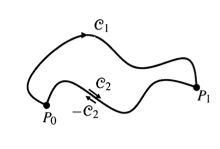
\includegraphics[scale=1]{image3.png}

Un dernier point :

Si l'on calcule tous les chemins possible entre $P_1$ et $P_0$ et qu'il y a indépendance de chemin, peut-on conclure que le champ de vecteur F est conservatif ?

La réponse est :" Ca dépend "

Mais la réponse est oui dans le cas où F est défini sur un domaine $D\subset \mathbb{R}^n$ ouvert et connexe
\begin{mydef}

Un domaine est connexe si quelque soit le couple de point $P_0$ et $P_1$, on peut trouver un chemin pour relier les deux points
\end{mydef}


Un exemple de domaine qui n'est pas connexe : \\
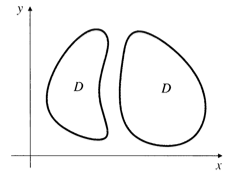
\includegraphics[scale=1]{image1.png}
\\
Un exemple de domaine connexe :
\\
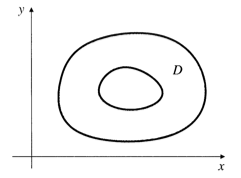
\includegraphics[scale=1]{image2.png}

\subsection{Démonstration constructive}

( C'est une démo qui explique comment calculer en plus de démontrer )

On considére dans l'espace de $\mathbb{R}^3$, un point P de coordonnées $P_0 = (x_0,y_0,z_0) $  et $P = (x,y,z)$

\[P_0, P \in D \text{ ouvert et connexe }\]

On définit $\Phi$ tel que

\[\Phi (x,y,z ) =\int_C F\bullet dr \]
où C est une courbe reliant $P_0$ à P

On a utilisé le fait que le domaine est connexe et qu'il y a indépendance des chemins.

On va montrer que \[\nabla \Phi = F \Longleftrightarrow F \text{conserv.} \]

\[\frac{\partial \Phi}{\partial x} \overset{?}{=} F_1 (x,y,z) \]

On peut trouver un point $P' = ( x_1,y,z)$ tel que $x_1 < x$ est dans le domaine. On est certain de le trouver comme le domaine est ouvert.

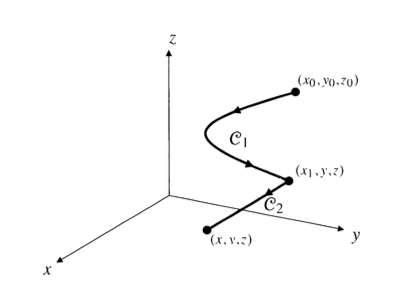
\includegraphics[scale=0.7]{image4.png}

\[C=C_1+C_2\]
\[\Phi (x,y,z) = \int_{C_1} F + \int_{C_2} F\]

On trouve que $\int_{C_1} F$ ne dépend pas de x. Donc $\frac{\partial I_1}{\partial x }=0$

\[x_1\leqslant t \leqslant x \]
\[r(t) = t i +yj + zk \]
\[dr = \frac{dr}{dt}dt = (dt)i\]

On a donc

\[I_C = \int_{x_1}^x (F\bullet i)dt = \int_{x_1}^x F_1 dt\] avec $F_1 = F_1 ( t,y,z )$

On vient de montrer que

\[\frac{\partial I_2	}{\partial x} = F_1 = \frac{\partial \Phi}{\partial x}\]


\begin{mytheo}

\textbf{A connaître}

Soit D ouvert connexe de $\mathbb{R}^n$ et F champ de vecteurs défini dans D. Il y a \emph{équivalence } des trois énoncés suivants.

\begin{itemize}
\item F est conservatif sur D, c'est-à-dire il existe un potentiel scalaire $\Phi$ tel que $F=\nabla \Phi $ dans D
\item $\oint_C F =0 \forall $ courbe fermée de D
\item $\forall P_0,P_1$ dans D, $\forall$ chemin C reliant $P_0$ et $P_1$ dans D
\end{itemize}
\[\int_C D \text{ a une valeure identique ( indépendance de chemin ) }\]

\end{mytheo}

\begin{mytheo}[Poincaré]
Connaissant F, puis-je facilement décider si F est ( ou non ) conservatif ? ( Sans essayer de trouver un potentiel $\Phi$ ni essayer de trouver une infinité de chemin )

Nous verrons plus loins que pour D simplement connexe, on peut ajouter un 4 ième énoncé.

$$\frac{\partial F_i}{\partial x_j} = \frac{\partial F_j}{\partial x_i}$$

Ce théorème est applicable uniquement si le domaine est simplement connexe.
\end{mytheo}

\begin{mydef}
$D$ simplement connexe ssi connexe et toute courbe fermée qui ne s'intersecte pas peut être  transformée continument en un point de D sans quitter $D$
\end{mydef}

Par exemple :

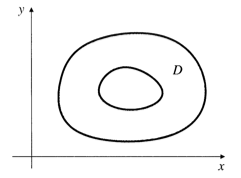
\includegraphics[scale=0.7]{image2.png}\\
n'est pas simplement connexe.
La fonction $ \Phi =xy^2 $  est le potentiel $F=y^2i+2xyj$ ( par définition, c'est un champ de vecteur conservatif. )

$F= yi-xj$, calculons, $\frac{\partial F_1}{\partial y} = 1 \neq \frac{\partial F_2}{\partial x} = -1$ En effet, pour qu'un champ de vecteur soit conservatif, il faut que ces deux dérivées partielles soient égales

Pour utiliser Poincaré, on doit d'abord vérifier que les hypothèses sont vérifiées.

\section{Le flux d'un champ de vecteur à travers une surface}

Cfr Adams 15.6\\

C'est une intégrale de Surface de la composaante normale à une surface d'un champ de vecteurs.

\subsection{Introduction}
 Surface orientée\\
 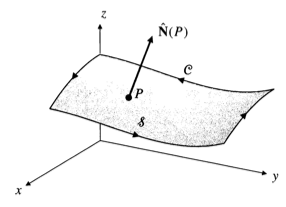
\includegraphics[scale=0.6]{image5.png}

 Le côté positif de la surface est le côté du vecteur normal tandis que le côté négatif, c'est l'autre.

 Par convention, l'orientation d'une surface induit une orientation particulière des bords de la surface ( s'ils existent )

 La règle est la suivante : on se met sur la face positive de S et on marche le long du bord C en laissant S à gauche, ce qui définit l'orientation positive de C.

 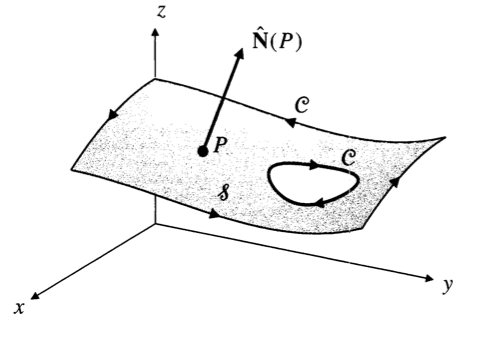
\includegraphics[scale=0.7]{image6.png}
 La face positive est au dessus et la face négative est en dessous. Par convention, les flèches représentent le sens de parcours positif.

 Voire ces exemples :

 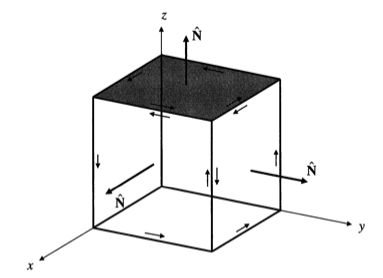
\includegraphics[scale=0.6]{image7.png}\\
 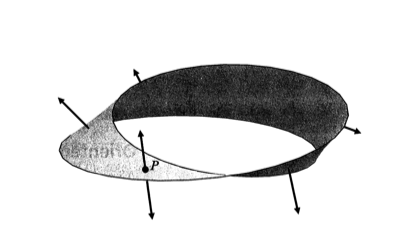
\includegraphics[scale=0.6]{image8.png}

 \subsection{Flux d'un champs vectoriel à travers une surface}

 On souhaite connaître la vitesse d'un cours d'eau à un endroit donné. On va placer une surface S fictive.\\

 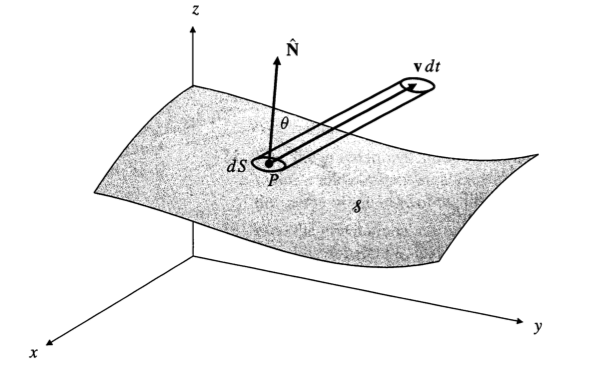
\includegraphics[scale=0.5]{image9.png} % Image 15.29
\\ On cherche le volume du cylindre. On pose $\rho \equiv 1$

 \[Vol = ||V||dt \cos \Theta dS\]

 avec $||V||dt \cos \Theta = V\bullet \hat N$


 Par unités de temps, la quantité de fluide qui passe à travers $dS$ est donc \[V(P) \bullet \hat N(P) dS\]

 \[\int_S \text{flux } dS = \text{ flux total de matière à travers S}\]

 \begin{mydef}
 Le flux d'un champ de vecteurF  à travers une surface orientée S est donnée par\[\int_S F \bullet \hat N ds = \int_S F \bullet dS\]

 et $F \bullet \hat N$ est la composante normale à S de F.

 avec $dS = \hat N dS$ élément de surface vectoriel

 Notation : $\int_C F$
 \end{mydef}

\begin{myrem}

$S$ fermée ( sphère ) :  $ \oiint_S F\bullet \dif S$

\[\oint F\bullet \dif r\]

\end{myrem}

Exemple : $F = (x) i + (y) j+(z) k$

Flux sortant du cylindre
\[\left\{
\begin{array}{c}
F=y^2i+2xyjx^2+y^2\leqslant a^2 \\
-h\leqslant z \leqslant h
\end{array}
\right.\]


La surface totale S : top+ buttom + coté

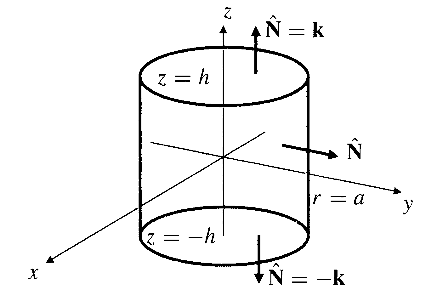
\includegraphics[scale=0.5]{image10.png}

\[\int_S F\bullet dS = \Sigma\text{flux}\]

On calcule sur chacune des faces.

\begin{enumerate}
  \item
    $z = +h$; $\hat N = k$ et  $dS= rd\Theta dr$

    \[\int_{top}F\bullet \hat N dS = \int_O^{2\pi} d\Theta \int_0â h r dr = \pi a^2 h\]

  \item $z = +h$; $\hat N = -k \Rightarrow =\pi a^2 h $

  \item coordonées cylindriques

    \[-h \leqslant z\leqslant h \] et aussi
    \[0\leqslant \Theta \leqslant 2 \pi\]

    $dS = ad\Theta dz$

    \[\vec{F} = (a\cos\Theta ) \hat i +(a\sin\Theta ) \hat j + z \hat k  \]

    \[\hat N = (\cos\Theta ) \hat i +a\sin\Theta ) \hat j\Leftrightarrow \vec F \hat N dS = a^2d\Theta dz\]
    \[\int_0^{2\pi} d\Theta \int_{-h}^{+h} a^2 dz = 4\pi a^2 h\]

\end{enumerate}

Le flux total vaut donc la somme de 1, 2 et 3 = $ 6 \pi a^2 h $

\fbox{
\begin{minipage}{10cm}
\textbf{Formule à connaître \# 5}

Règle de calcul


$r(u,v)$ de $S$ avec $(u,v^\in D\subset \mathbb{R}^2$

On a vu que :
\begin{itemize}
\item
$n=\frac{\partial r}{\partial u } \times \frac{\partial r}{\partial v }$

normal à S ( Par définition du produit vectoriel )

\[\hat N = \pm \frac{n}{||n||}\]
le $\pm$ dépend de notre choix d'orientation de S
\item
\[ dS = ||n||dudV \]
\end{itemize}

On a donc
\[ dS = \hat N dS = \pm\frac{n}{||n||}dudv = \pm
n \dif u \dif v \]

et finalement, $F=F_1(x,y,z)i+F_2(x,y,z)j+F_3(x,y,z)k$

Flux de S à travers S est donné par

\[\int_S F\bullet dS = \pm \int_D F\bullet \left(\frac{\partial r}{\partial u } \times \frac{\partial r}{\partial v } \right) dudv\]


 Cette formule nous permet de calculer l'intégrale d'un champ vectoriel à travers une surface.
\end{minipage} }

$$
\text{Flux} = \pm \int \left(F_1( x(u,v),y(u,v),z(u,v) )\frac{\partial(y,z)}{\partial (u,v)} \right.
$$

$$
+F_2( x(u,v),y(u,v),z(u,v)(\frac{\partial(z,x)}{\partial (u,v)}
$$

$$\left.+F_3( x(u,v),y(u,v),z(u,v)(\frac{\partial(x,y)}{\partial (u,v)}\right) dudv
$$

avec par exemple

\[\frac{\partial(z,x)}{\partial (u,v)}=\frac{\partial z}{\partial u}\frac{\partial x}{\partial v}-\frac{\partial z}{\partial v}\frac{\partial x}{\partial u}\]

et \[\vec r (u,v) = x(u,v)\hat i +y(u,v)\hat j +z(u,v)\hat k \]
